\documentclass[notheorems]{beamer}
\setbeamertemplate{caption}[numbered]
%\usepackage{subfig}
\usepackage[ruled,vlined,spanish]{algorithm2e}
\usepackage{amsthm}
\usepackage{amssymb}
\usepackage{array}
\usepackage[spanish]{babel}
\usepackage{blkarray}
\usepackage{bm}
\usepackage{booktabs}
\usepackage[font=footnotesize]{caption}
\usepackage{float}
\usepackage{graphicx}
\usepackage[utf8]{inputenc}
\usepackage{mathtools}
\usepackage{setspace}
\usepackage{subcaption}
\newcommand{\figura}[3]{\begin{figure}[H] \centering \includegraphics[#3]{#1} \caption{#2} \label{#1}  \end{figure}}
\newcommand{\tablasimple}[2]{\begin{table}[H] \centering \input{#1} \caption{#2} \label{#1} \end{table}}
\newcommand{\tablalarga}[2]{ \begin{center} \input{#1} \begin{table}[H] \caption{#2} \label{#1} \end{table} \end{center}}
\usetheme{CambridgeUS}
\usecolortheme{seahorse}
\institute[]{Statistical Machine Learning \\ Profa. Guillermina Eslava \\ Posgrado en Ciencias Matemáticas \\ Universidad Nacional Autónoma de México}
\author{César Cossio Guerrero. Aldo Sayeg Pasos Trejo}
\date{\today}
\title[Proyecto final]{Proyecto final: Redes Neuronales}
\begin{document}

\begin{frame}
    \maketitle
\end{frame}
\begin{frame}{Análisis exploratorio}
    \figura{digits.pdf}{Muestra de tres imágenes que comprenden el conjunto de datos MNIST}{width = 0.55\textwidth}
    \figura{hist.pdf}{Histogramas de proporción de clase para los conjuntos de entrenamiento y prueba}{width = 0.55\textwidth}
\end{frame}
\begin{frame}{Batch size}
    \begin{figure}[h]
        \centering
        \begin{subfigure}[c]{0.40\textwidth}
            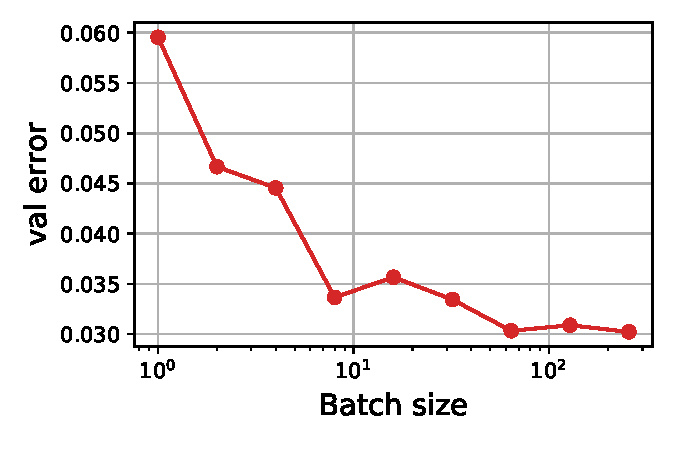
\includegraphics[width=\textwidth]{batchSizeAnalError.pdf}
            \caption{}
            \label{fig:bsError}
        \end{subfigure}
        \begin{subfigure}[c]{0.4\textwidth}
            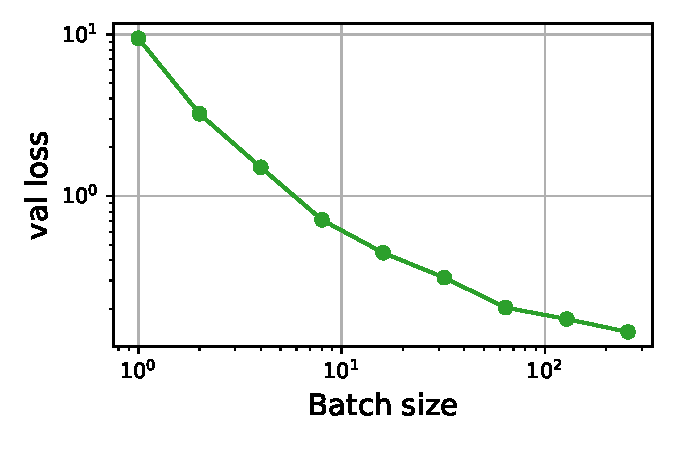
\includegraphics[width=\textwidth]{batchSizeAnalLoss.pdf}
            \caption{}
            \label{fig:bsLoss}
        \end{subfigure}
        \caption{Error y funcion de perdida como función del batch size. El error se presenta en tasa}
    \end{figure}
\end{frame}
\begin{frame}{Regresión Logistica}
    
    \begin{table}[H]
        \centering
        \begin{tabular}{c|c|c|c}
            \toprule
            error & val error & cv val error mean & cv val error std \\
            \midrule
            6.0500 &  7.8000 & 7.7650 & 0.1977  \\
            \bottomrule
        \end{tabular}
        \caption{Porcentajes de error para la regresión logística. Los errores de validación cruzada se obtuvieron para $k=5$ folds y una sola repetición.}
        \label{tab:logreg}
    \end{table}
\end{frame}
\begin{frame}
    \frametitle{Modelos DNN}
    \begin{table}[H]
        \centering
        \resizebox{\textwidth}{!}{
        \begin{tabular}{c| p{1.5cm}| p{1cm}| p{2cm}| p{3cm}| p{2.5cm} | p{1.5cm}| p{1cm}}
            \toprule
            Name &  Trainable Parameters &  Dense Layers & Nodes per Layer &  Activation Functions &  Regularization & Dropout & Input Dropout \\
            \midrule
            DNN1 &  318010 & 1 & [400] & [tanh] & [0] & [0.1] & 0.5 \\
            DNN2 &  178110 & 2 & [200, 100] & [tanh, swish] & [0.005,0.001] & [0,0] & 0.2 \\
            DNN3 &  178110 & 2 & [200, 100] & [tanh, tanh] & [0.005,0.001] & [0,0] & 0.2 \\
            DNN4 &  188210 & 3 & [200, 100, 100] & [tanh, tanh, tanh] & [0.001, 0,0] & [0,0,0] & 0.2 \\
            DNN5 &  203260 & 3 & [200, 150, 100] & [tanh, relu, tanh] & [0.001, 0,0] & [0,0,0] & 0.2 \\
            DNN6 &  213360 & 4 & [200, 150, 100, 100] & [tanh, swish, tanh, swish] & [0.001, 0,0,0] & [0,0,0,0] & 0.2 \\
            \bottomrule
        \end{tabular}}
        \caption{Descripción de los seis modelos DNN. La columna Dropout indica el valor del dropout después de la capa densa. Input Dropout es la fracción de dropout entre la entrada de datos y la primera capa densa. La columna Regularization indica la regularización sobre las aristas posteriores a cada capa densa.}
        \label{tab:DNNdes}
    \end{table}
\end{frame}
\begin{frame}
    \frametitle{Modelos DNN}
    \begin{table}[H]
        \centering
        \resizebox{\textwidth}{!}{
        \begin{tabular}{c| p{1.5cm}| p{1.5cm}| p{1.5cm}| p{1.5cm}| p{1.5cm}| p{1.5cm}| p{1.5cm}| p{1.5cm}}
            \toprule
            Name &  error &  val error &  cv val error mean &  cv val error std &  loss &  val loss &  cv val loss mean &  cv val loss std \\
            \midrule
            DNN1 &  1.935 &      2.367 &              4.930 &             0.256 & 0.058 &     0.104 &             0.159 &            0.010 \\
            DNN2 &  0.000 &      2.444 &              2.997 &             0.382 & 0.000 &     0.342 &             0.662 &            0.156 \\
            DNN3 &  0.972 &      2.633 &              3.380 &             0.169 & 0.033 &     0.193 &             0.161 &            0.013 \\
            DNN4 &  1.342 &      2.622 &              8.470 &             0.544 & 0.355 &     0.390 &             1.351 &            0.050 \\
            DNN5 &  1.152 &      2.544 &              8.077 &             0.609 & 0.368 &     0.432 &             1.336 &            0.031 \\
            DNN6 &  1.050 &      2.533 &              8.055 &             0.899 & 0.358 &     0.406 &             1.366 &            0.040 \\
            \bottomrule
            \end{tabular}}
            \caption{Errores y función de pérdida para las redes DNN. Los errores se muestran en porcentaje}
            \label{tab:DNNres}
    \end{table}
\end{frame}
\begin{frame}
    \frametitle{Modelos CNN}
    \begin{figure}[H]
        \begin{center}
            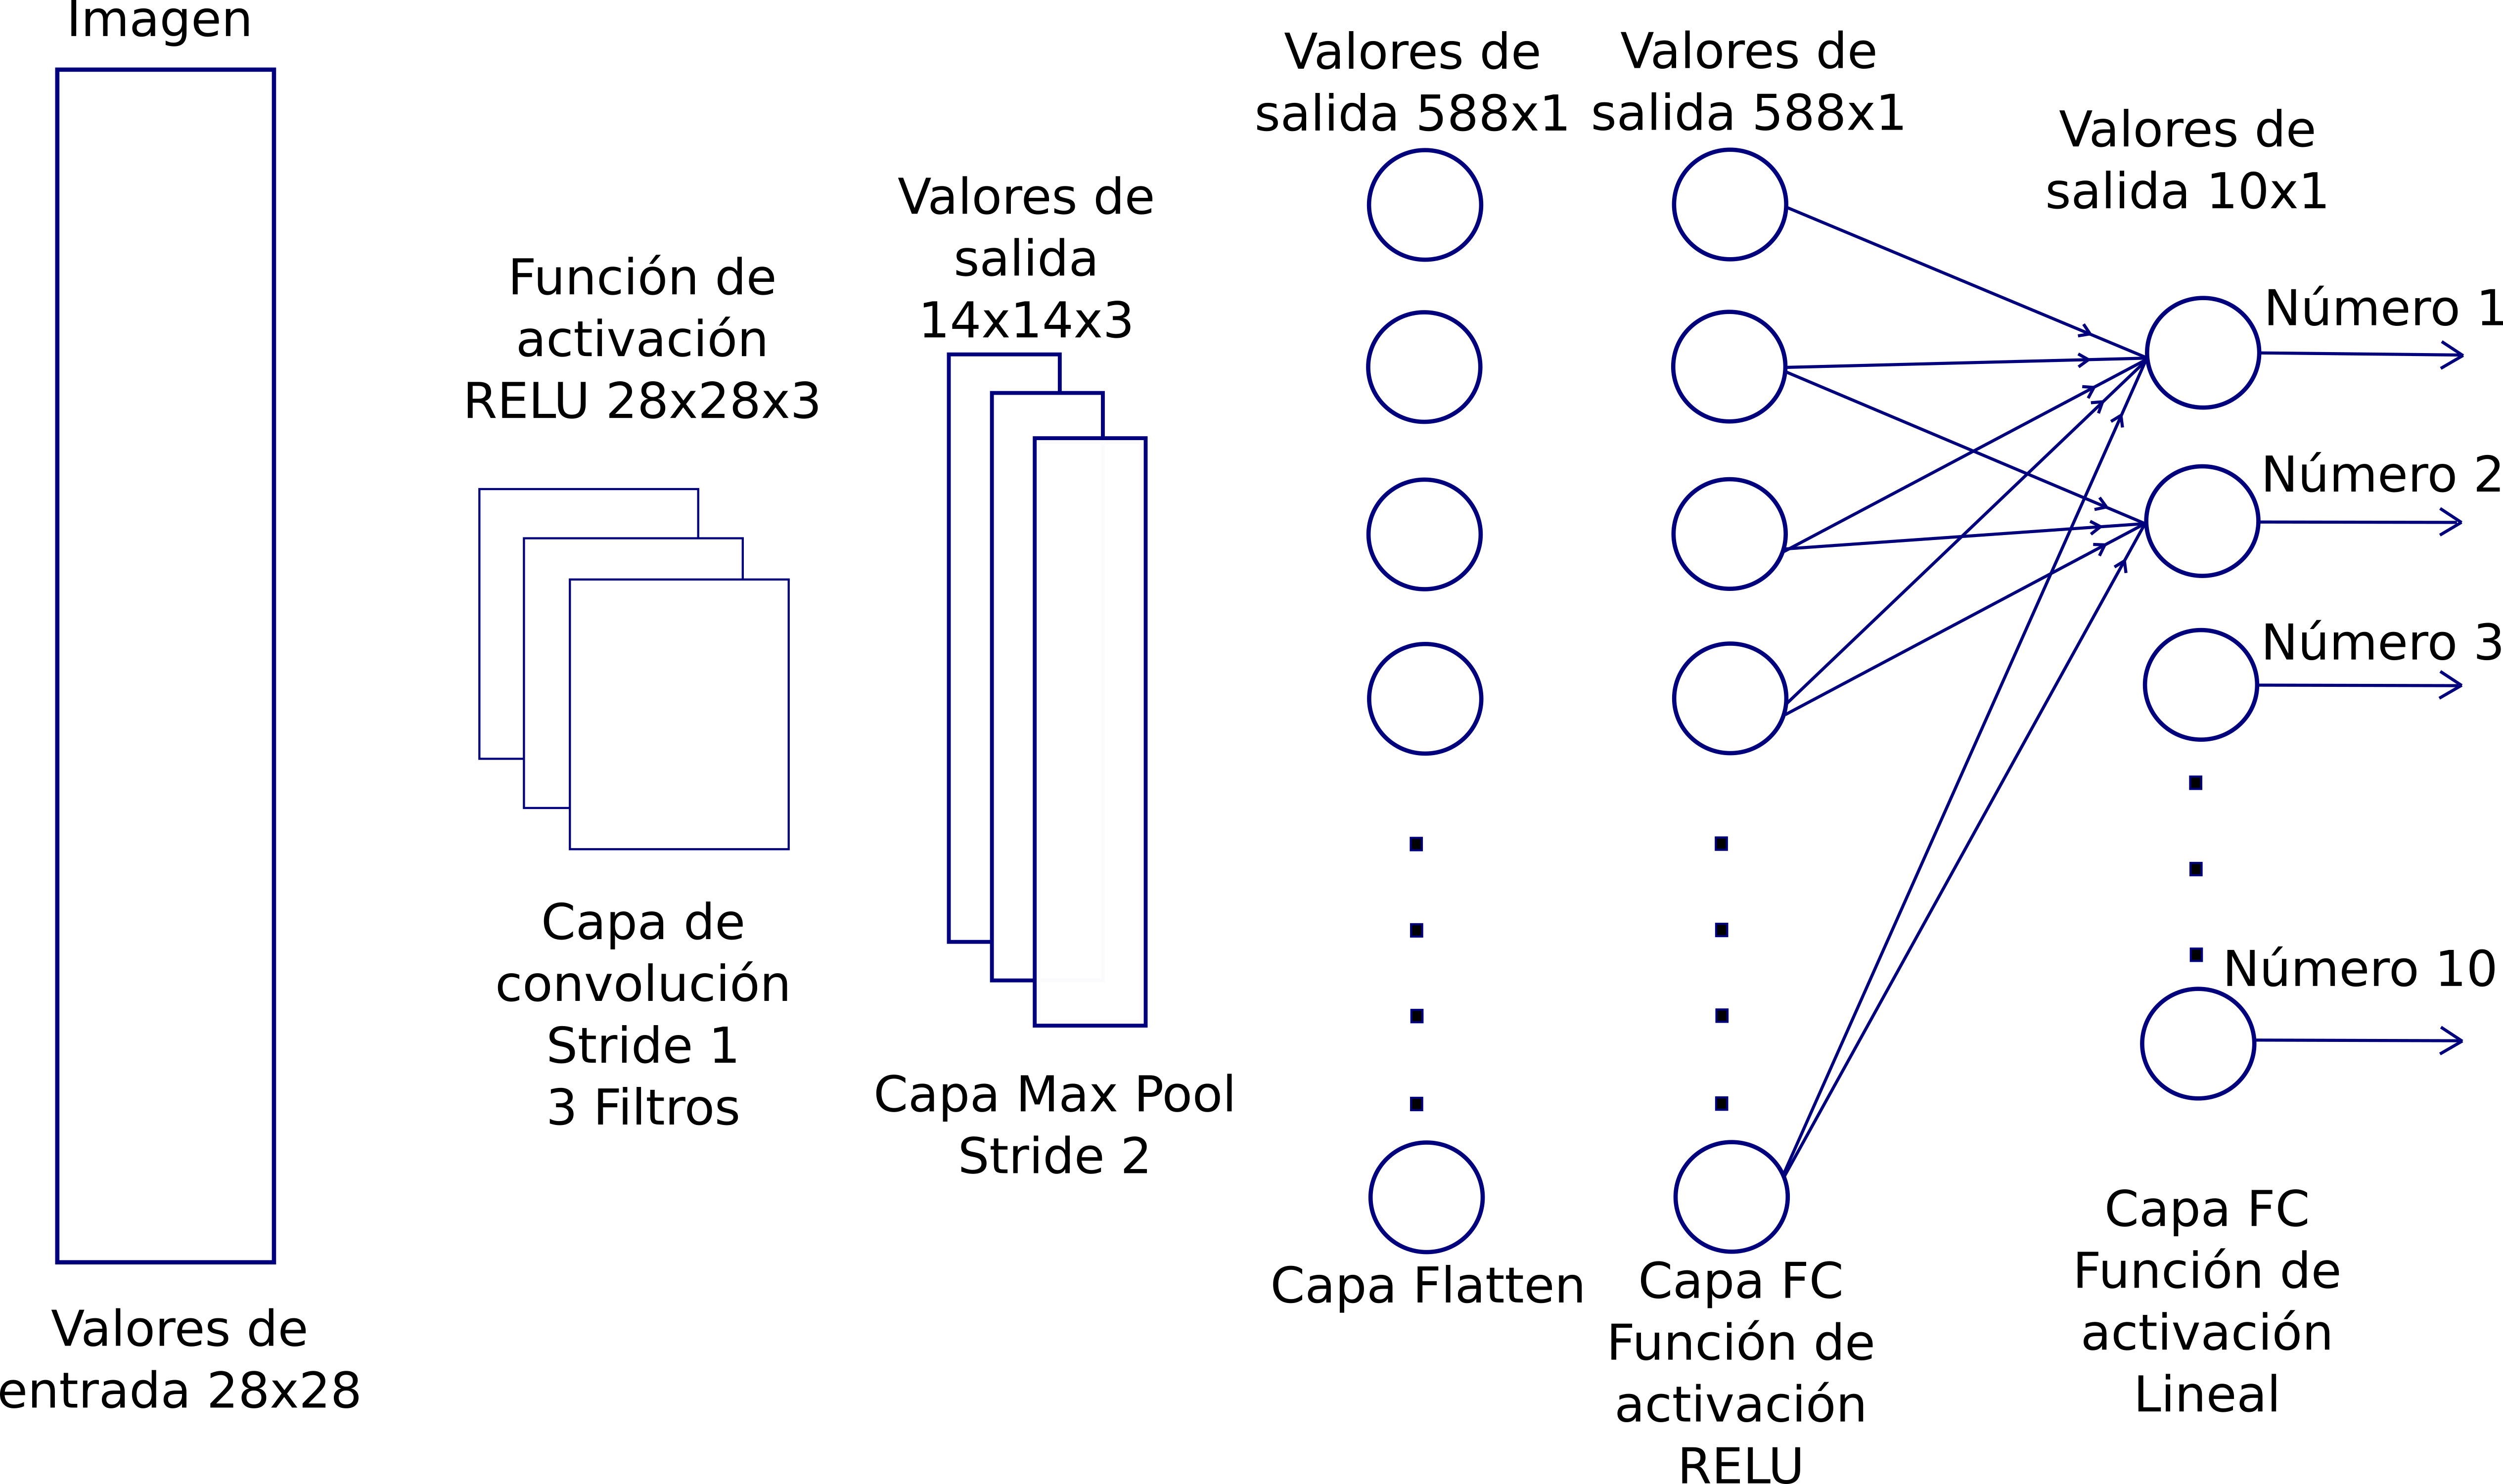
\includegraphics[width = 0.85\textwidth]{ArquitecturaINK2.png}
        \end{center}
        \caption{Esquema de la arquitectura básica de una CNN. .}
        \label{fig:ES-CN}
    \end{figure}
\end{frame}
\begin{frame}{Modelos CNN}
    \begin{table}[H]
        \centering
        \resizebox{\textwidth}{!}{
        \begin{tabular}{c| p{1.5cm}| p{1.5cm}| p{1.5cm}| p{1.5cm}|  p{1.5cm}|  p{2.2
        cm} | p{1.5cm} | p{1.5cm}}
            \toprule
            Name &  Trainable Parameters &  Dense Layers &  Conv. Layers &  Nodes per Layer & Activation Functions &  Regularization & Dropout & Input Dropout \\
            \midrule
            CNN1 & 542230 & 1 & 1 &  [100] & [relu] & [0] & [0] & [0] \\
            CNN2 & 542230 & 1 & 1 &  [100] & [relu] & [0] & [0] & [0.5] \\
            CNN3 & 179926 & 1 & 2 &  [100] & [relu] & [0] & [0] & [0] \\
            CNN4 & 180118 & 1 & 2 &  [100] & [relu] & [0] & [0] & [0.5] \\
            CNN5 & 209430 & 1 & 3 &  [100] & [relu] & [0] & [0] & [0] \\
            CNN6 & 209430 & 1 & 3 &  [100] & [relu] & [0] & [0] & [0] \\
            \bottomrule
        \end{tabular}}   
        \caption{Descripción sintetizada de los modelos de redes convolucionales}
        \label{tab:CNNdes}
    \end{table}
\end{frame}
\begin{frame}{Modelos CNN}
    \begin{table}[H]
        \centering
        \resizebox{\textwidth}{!}{
        \begin{tabular}{c| p{1.5cm}| p{1.5cm}| p{1.5cm}| p{1.5cm}| p{1.5cm}| p{1.5cm}| p{1.5cm}| p{1.5cm}}
            \toprule
            Name &  error &  val error &  cv val error mean &  cv val error std &   loss &  val loss &  cv val loss mean &  cv val loss std \\
            \midrule
            CNN1 & 0.0000 & 1.6556 & 2.6675 &            0.1904 & 0.0000 &    0.1768 &            0.2766 &           0.0314 \\
            CNN2 & 0.2875 & 1.7667 & 2.1700 &            0.3061 & 0.0098 &    0.1243 &            0.1127 &           0.0187 \\
            CNN3 & 0.0000 & 1.1222 & 1.7900 &            0.0987 & 0.0000 &    0.0857 &            0.2167 &           0.0825 \\
            CNN4 & 0.2575 & 0.8889 & 0.9050 &            0.1171 & 0.0078 &    0.0478 &            0.0535 &           0.0138 \\
            CNN5 & 0.1600 & 0.7222 & 0.9000 &            0.1951 & 0.0051 &    0.0458 &            0.0612 &           0.0153 \\
            CNN6 & 1.7055 & 0.7889 & 0.6950 &            0.0911 & 0.0553 &    0.0313 &            0.0237 &           0.0051 \\
            \bottomrule
            \end{tabular}}
        \caption{Errores y función de pérdida para las redes CNN. Los errores se muestran en porcentaje}
        \label{tab:CNNres}        
    \end{table}
\end{frame}
\begin{frame}{Discusión}
    \begin{table}[H]
    \centering
    \resizebox{!}{0.35\textheight}{
    \begin{tabular}{c| p{1.5cm}| p{1.5cm}| p{2cm}| p{1.5cm}}
        \toprule
        Name &  Trainable Parameters &  Dense Layers &  Convolution Layers &  execution  time (hours) \\
        \midrule
        Log & 7850 & - & - & 13.2 \\
        DNN1 &                318010 &             1 &                   0 &                   0.7020 \\
        DNN2 &                178110 &             2 &                   0 &                   0.7002 \\
        DNN3 &                178110 &             2 &                   0 &                   0.7146 \\
        DNN4 &                188210 &             3 &                   0 &                   0.7586 \\
        DNN5 &                203260 &             3 &                   0 &                   0.7545 \\
        DNN6 &                213360 &             4 &                   0 &                   0.7988 \\
        CNN1 &                542230 &             1 &                   1 &                   0.4366 \\
        CNN2 &                542230 &             1 &                   1 &                   0.4467 \\
        CNN3 &                179926 &             1 &                   2 &                   0.4867 \\
        CNN4 &                180118 &             1 &                   2 &                   0.5449 \\
        CNN5 &                209430 &             1 &                   3 &                   0.6473 \\
        CNN6 &                209430 &             1 &                   3 &                   0.9363 \\
        \bottomrule
    \end{tabular}}
    \caption{Descripción sintetizados de los modelos de redes neuronales}
    \label{tab:fullDescrip}
\end{table}
\end{frame}
\begin{frame}{Discusión}
    \begin{table}[H]
        \resizebox{\textwidth}{!}{
        \begin{tabular}{c| p{1.5cm}| p{1.5cm}| p{1.5cm}| p{1.5cm}| p{1.5cm}| p{1.5cm}| p{1.5cm}| p{1.5cm}}
            \toprule
            Name &  error &  val error &  cv val error mean &  cv val error std &   loss &  val loss &  cv val loss mean &  cv val loss std \\
            \midrule
            Log  & 6.0500 &     7.8000 &             7.7650 &            0.1977 & - & - & - & - \\ 
            DNN1 & 1.9350 &     2.3667 &             4.9300 &            0.2563 & 0.0577 &    0.1036 &            0.1586 &           0.0101 \\
            DNN2 & 0.0000 &     2.4444 &             2.9975 &            0.3816 & 0.0000 &    0.3416 &            0.6622 &           0.1558 \\
            DNN3 & 0.9725 &     2.6333 &             3.3800 &            0.1691 & 0.0331 &    0.1929 &            0.1605 &           0.0131 \\
            DNN4 & 1.3425 &     2.6222 &             8.4700 &            0.5439 & 0.3547 &    0.3901 &            1.3511 &           0.0499 \\
            DNN5 & 1.1525 &     2.5444 &             8.0775 &            0.6088 & 0.3680 &    0.4323 &            1.3359 &           0.0314 \\
            DNN6 & 1.0500 &     2.5333 &             8.0550 &            0.8987 & 0.3582 &    0.4060 &            1.3664 &           0.0401 \\
            CNN1 & 0.0000 &     1.6556 &             2.6675 &            0.1904 & 0.0000 &    0.1768 &            0.2766 &           0.0314 \\
            CNN2 & 0.2875 &     1.7667 &             2.1700 &            0.3061 & 0.0098 &    0.1243 &            0.1127 &           0.0187 \\
            CNN3 & 0.0000 &     1.1222 &             1.7900 &            0.0987 & 0.0000 &    0.0857 &            0.2167 &           0.0825 \\
            CNN4 & 0.2575 &     0.8889 &             0.9050 &            0.1171 & 0.0078 &    0.0478 &            0.0535 &           0.0138 \\
            CNN5 & 0.1600 &     0.7222 &             0.9000 &            0.1951 & 0.0051 &    0.0458 &            0.0612 &           0.0153 \\
            CNN6 & 1.7055 &     0.7889 &             0.6950 &            0.0911 & 0.0553 &    0.0313 &            0.0237 &           0.0051 \\
            \bottomrule
            \end{tabular}}
            \caption{Estadísticas de pérdida para los modelos. El modelo ``Log'' corresponde a la regresión logística. Las tasas de error están presentadas en porcentaje}
        \label{tab:fullErrors}
    \end{table}
\end{frame}
\begin{frame}{Discusión}
    \figura{modelsPlot.pdf}{Comparación gráfica entre los 12 modelos escogidos. El error se muestra en tasa}{width = 0.8\textwidth}
\end{frame}
\begin{frame}{Discusión}
    \figura{modelsGrid.pdf}{Error de entrenamiento y validación como función de la época para los doce modelos entrenamos. Los modelos CNN fueron entrenados por 50 épocas mientras que los de DNN fueron entrenados por 100}{height=0.7\textheight}
\end{frame}
\begin{frame}{Discusión}
    \begin{table}[h!]
        \resizebox{\textwidth}{!}{
        \centering
        \begin{tabular}{c| p{1.5cm}| p{1.5cm}| p{1.5cm}| p{1.5cm}| p{2cm}| p{1.5cm}| }
            \toprule
            Name &  error &  val error &  cv val error mean &  cv val error std & parameters & execution time \\
            \midrule
            Log  & 6.0500 &     7.8000 &             7.7650 &            0.1977 &  7850 & 13.2 \\ 
            CNN5 & 0.1600 &     0.7222 &             0.9000 &            0.1951 & 209430 & 0.6473 \\
            \bottomrule
            \end{tabular}}
            \caption{Comparación entre el modelo CNN5 y el modelo de regresión logística}
        \label{tab:finalCompar}
    \end{table}
\end{frame}
\begin{frame}{Discusión}
    \figura{crossValGrid.pdf}{Error de entrenamiento y validación para la versión principal como para las 10 iteraciones por Cross Validation para el modelo CNN5}{height=0.7\textheight}
\end{frame}
\begin{frame}{Discusión}
    \begin{table}[h]
        \centering
        \resizebox{!}{0.35\textheight}{
        \begin{tabular}{lrrrr}
        \toprule
        Conjunto &     error &  val error &  cv val error mean &  cv val error std \\
        \midrule
        Clase 0 &  0.0000 &   0.0000 &           0.1826 &          0.0032 \\
        Clase 1 &  0.0223 &   0.6869 &           0.8696 &          0.0154 \\
        Clase 2 &  0.0000 &   0.6593 &           0.8420 &          0.0149 \\
        Clase 3 &  0.0000 &   0.8483 &           1.0310 &          0.0182 \\
        Clase 4 &  0.0255 &   0.8018 &           0.9845 &          0.0175 \\
        Clase 5 &  0.0549 &   0.8696 &           1.0522 &          0.0186 \\
        Clase 6 &  0.0254 &   0.4429 &           0.6256 &          0.0111 \\
        Clase 7 &  0.0481 &   1.0822 &           1.2649 &          0.0224 \\
        Clase 8 &  0.0259 &   1.1312 &           1.3138 &          0.0233 \\
        Clase 9 &  0.0000 &   0.7067 &           0.8893 &          0.0157 \\
        Global & 0.1600 &     0.7222 &             0.9000 &            0.1951 \\
        \bottomrule
        \end{tabular}}
        \caption{Errores por clase y global para el conjunto de entrenamiento, prueba y para validación cruzada del modelo CNN5}
        \label{tab:classError}
    \end{table}
\end{frame}
\begin{frame}{Conclusiones}
    
\end{frame}
\end{document}